\documentclass[12pt]{article}
\usepackage[a4paper]{geometry}
\usepackage[estonian, english]{babel}
\usepackage[T1]{fontenc}
\usepackage{amsmath}
\usepackage{amsthm}
\usepackage{amssymb}

\usepackage{hyperref}
\usepackage{graphicx}
\usepackage{float}
\usepackage{epstopdf}
\usepackage{listings}

\usepackage{graphicx}
\graphicspath{{Figures/}}

% Packages for building tables and tabulars
\usepackage{array}

\usepackage{proof}
\usepackage{semantic}
\usepackage{commath}
\DeclareMathOperator{\sign}{sign}

% Packages for defining colourful text together with some colours
\usepackage{color}
\usepackage{xcolor}
%\definecolor{dkgreen}{rgb}{0,0.6,0}
%\definecolor{gray}{rgb}{0.5,0.5,0.5}
\definecolor{mauve}{rgb}{0.58,0,0.82}


% Standard package for drawing algorithms
% Since the thesis in article format we must define \chapter for
% the package algorithm2e (otherwise obscure errors occur)
\let\chapter\section
\usepackage[ruled, vlined, linesnumbered]{algorithm2e}

% Fix a  set of keywords which you use inside algorithms
\SetKw{True}{true}
\SetKw{False}{false}
\SetKwData{typeInt}{Int}
\SetKwData{typeRat}{Rat}
\SetKwData{Defined}{Defined}
\SetKwFunction{parseStatement}{parseStatement}


% Proper way to create coloured code listings
\usepackage{listings}
\lstset{
  %language=python,                % the language of the code
  language=C++,
  basicstyle=\footnotesize,        % the size of the fonts that are used for the code
  %numbers=left,                   % where to put the line-numbers
  %numberstyle=\footnotesize,      % the size of the fonts that are used for the line-numbers
  numberstyle=\tiny\color{gray},
  stepnumber=1,                    % the step between two line-numbers. If it's 1, each line
                                   % will be numbered
  numbersep=5pt,                   % how far the line-numbers are from the code
  backgroundcolor=\color{white},   % choose the background color. You must add \usepackage{color}
  showspaces=false,                % show spaces adding particular underscores
  showstringspaces=false,          % underline spaces within strings
  showtabs=false,                  % show tabs within strings adding particular underscores
  frame = lines,
  %frame=single,                   % adds a frame around the code
  rulecolor=\color{black},       % if not set, the frame-color may be changed on line-breaks within
                                   % not-black text (e.g. commens (green here))
  tabsize=2,                       % sets default tabsize to 2 spaces
  captionpos=b,                    % sets the caption-position to bottom
  breaklines=true,                 % sets automatic line breaking
  breakatwhitespace=false,         % sets if automatic breaks should only happen at whitespace
  %title=\lstname,                 % show the filename of files included with \lstinputlisting;
                                   % also try caption instead of title
                                   % also try caption instead of title
  keywordstyle=\color{blue},       % keyword style
  commentstyle=\color{dkgreen},    % comment style
  stringstyle=\color{mauve},       % string literal style
  escapeinside={\%*}{*)},          % if you want to add a comment within your code
  morekeywords={*,game, fun}       % if you want to add more keywords to the set
}



%%% BEGIN DOCUMENT
\begin{document}

% BEGIN TITLE PAGE
\thispagestyle{empty}
\begin{center}

\large
UNIVERSITY OF TARTU\\[2mm]
\uppercase{Faculty of Mathematics and Computer Science}\\[2mm]
Institute of Computer Science\\
%Specialty of Computer Science\\[2mm]

%\vspace*{\stretch{5}}
\vspace{25mm}

\Large Stenver Jerkku

\vspace{4mm}

\huge Paralell Wilcoxon Signed-rank tests

%\vspace*{\stretch{7}}
\vspace{20mm}

\Large Bachelor's Thesis (6 ECTS)

\end{center}

\vspace{2mm}

\begin{flushright}
 {
 \setlength{\extrarowheight}{5pt}
 \begin{tabular}{r l}
  \sffamily Supervisor: & \sffamily Sven Laur, PhD
 \end{tabular}
 }
\end{flushright}

%\vspace*{\stretch{3}}
\vspace{10mm}

%{\noindent Author: .................................................................................... ``.....'' ..........\hskip16pt 2048}
\vspace{2mm}


%{\noindent Supervisor: ............................................................................... ``.....'' ..........\hskip16pt 2048}

\vspace{2mm}

%{\noindent Supervisor: ............................................................................... ``.....'' ..........\hskip16pt 2048}

\vspace{8mm}

\vfill
\centerline{Tartu 2012}

\newpage


\begin{abstract}
Wilcoxon Signed-rank test is a paired statistical test that is used when measurement values are not normally distributed. The test is used by BIIT(Bioinformatics, Algorithmics and Data mining group) research group for gene regulation, gene expression data analysis, biological data mining and others. BIIT is joint research group between the Department of Computer Science (University of Tartu), Quretec, and the Estonian Biocenter.

The current implementations of the Wilcoxon Signed-rank tests are slow and unoptimized. This project will look into the foundations of wilcoxon signed-rank test, its current implementations and how to optimize it. In order to make the implementation more accurate, the relationship between Wilcoxon statistic and Guassian approximate will be observed. In order to make the implementation faster, some dynamic programming methods will be used to save computation time. The goal of optimizing is to make it more accurate and speed up the test running.

The end goal of this project is to create an accurate and fast wilcoxon test implementation in C++ shared library. In the scope of this project, the library will be integrated with two tools -command line and Cron-R. Due to the nature of shared library, it will be easy integrate the library with any other tools one might desire.

\end{abstract}

\newpage

\tableofcontents

\newpage

\section{Introduction}
The BIIT research group has biologist who conduct a variety of experiments on a control group. They try to measure, compare and test different attributes of a living organism. These attributes might be, but not limited to blood pressure, proteine amount in the blood, RNA amount, purity of urine, brainwaves etc. These attributes can be repeadedly measured on the same subject and the results are never exactly the same. There is always a little noise and varience between the samples. Biologist often experiment on the control group and try to affect these observed attributes. The take samples before and after simulating the observable attribute with some stimulant. This is called the case-control study.

However, since even without external stimulation the two results are never the same. Also, different experiments can have wildly different assumptions, so you cannot simply use a constant error margin on all your tests. For example, the blood pressure measuring before and after jogging could have a lot bigger changes then brainwave changes.  Therefore  the biologist need to use statistical tests to find out which case-control studies are actually significant and which are simply noise.

There are many case-control tests available. For example paired Students t-test, t-test for matched pairs and Wilcoxon signed-rank test. The Wilcoxon signed-rank test is used when the measurement values are not normally distributed when the experimental conditions are fixed.  In practise, this means that the histogram of measurements is either asymmetrical or it does not resemble the bell shape.

It is common to assume that properly scaled gene expression measurements follow Gaussian distribution, while quantities of proteins and metabolites are assumed to have non-gaussian distribution.

\subsection{NetCDF file format}
The BIIT group holds statistical data in NetCDF file format. NetCDF is an open source standard of a set of data formats, programming interfaces, and software libraries that help read and write scientific data files. \url{http://www.unidata.ucar.edu/software/netcdf/docs/what_is_netcdf.html}$^2$
Data can be held in a structured manner in a NetCDF file. You can define dimensions, name them, put variables in the dimensions and later retrieve or change them. This is useful, for example, to hold matrix like data in a file and have fast lookups. In addition, you can define helper dimensions for the matrix for extra information.
NetCDF file format is used by the BIIT researh group to hold gene data and will be given as an input file for the program.

Currently the BIIT group holds the data in the NetCDF file in the following format:

\textbf{Data matrix}
\begin{itemize}
  \item double data(m, n) - the data matrix of m genes (variables) and n samples (experiments, patients, ...)
  \item string gene[m] - gene IDs
  \item string array[n] - sample IDs
\end{itemize}

\textbf{Non-track metadata}
\begin{itemize}
  \item string \_\_FileFormat - EVDF format identifier string. Current value: "ExpressView 1.1".
  \item string \_\_DatasetType - A string identifying the dataset type. This is used to extract data-specific parameters from a global configuration file. See datatypes.conf (ExpressViewConfigFiles) for allowed values.
  \item string[n] Organism - Organism (per column)
  \item string[n] MetadataOrder - Sometimes metadata (including column tracks) may be in a different order than columns in data. This variable is a permutation of the array variable, specifying the order of column variables. This field is deprecated and all column metadata is expected to be in array order in new datasets.
  \item string InvestigationTitle - short title for the dataset
  \item string ExperimentDescription - long description for the dataset
  \item string DatasetID - Optional Source-specific dataset identifier
  \item string DatasetLink - Optional A URL associated with the dataset
  \item string \_\_VariableLabel - Optional Custom variable type name for the dataset. Overriden by variable\_label in project configuration. (ExpressView)
Names of any other (optional, non-track) metadata variables must be prepended by two underscores. Additional variables may be mandated by a data type specification, see ExpressViewConfigFiles. Known specific variables:
  \item string \_\_Organism - ArrayExpress chip organism (ArrayExpress; as opposed to the source of biological material stored in Organism)
\end{itemize}

\textbf{Tracks}

Tracks are all other variables whose name begins with an uppercase character, that are arrays of either string or double, with the size of their first dimension either m or n. The former are referred to asrow tracks and the latter as column tracks. These variables encode some information about either the rows or columns of the data matrix; e.g. ExpressView displays column tracks above the heatmap.

Examples:

string Chemotherapy[n]
string Local\ Relapse[n]
double RelativeVariance[m]

\subsection{Current BIIT procedures}
Currently the BIIT group has 3 ways of analysing its data.
\subsubsection{GNU R}
They can use GNU R project to make custom and complext analyses. For that they need to manually read NetCDF file to the R and then call the R built in function wilcox.test to use Wilcoxon test. The problem with R wilcoxon test is that it is slow. If you run thousands of tests in a row, the results might come after hours of computer processing. One of the goals of this paper and project is to make Wilcoxon test run on command line in mere seconds.
\subsubsection{Web interface}
They can use a web interface which can take in certain arguments and command line script. It then will use whatever command line tools it has available and visualizes the output.

\subsubsection{Command line}
They can also use the command line directly which has a variety of tools installed. The wilcoxon test will ultimately call R wilcoxon function.

So in the end - no matter how the biologist analyse their data, they will always use wilcoxon test in the GNU R project.

\newpage

\section{Wilcoxon signed-rank test}

In this section, we discuss a particular statistical test called Wilcoxon signed-ran test. Wilcoxon test can be used to make sure that something has an effect on the measured samples. For example, biologist could measure 3 patients white blood cell levels, create some external stimulation on the patients and measure the white blood cell levels again. The wilcoxon signed-ranked test shows wether the external stimulation had any statistical effect on the white blood cell levels.
\subsection{Statistical Tests}

The statistical tests are usually done, because initial research has raised a hypothesis about the data. It is desireable to know if the hypothesis is true or not.

\begin{figure}[!ht]
  \centering
  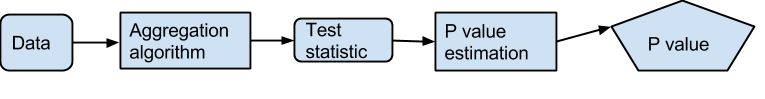
\includegraphics[width=0.8\textwidth]{statisticalTestFlow}
  \caption{Graphical represenation of statistical test flow}
  \label{fig:statisticalTestFlow}
\end{figure}

Statistical tests are usually built by first gathering the necessary raw data. For example, make 80 persons run for 30 minutes and measure blood pressure before and after running. The data is then organized by some kind of aggregation algorithm which also might filter out samples that are not related to the hypothesis in question. For example, sorting and grouping the blood pressure results by gender, weight and in ascending order and then filter out any group that had too few samples. Then a test statistic is chosen and calculated. After that a p-value can be estimated which tells if the observable feature is interesting or not. For example, if running plays a role in raising a persons blood pressure.

\subsubsection{Test Statistic}

The test statistic is a scalar function of all the observations, which summarizes the data by a single number. This value is used to estimate a p-value and accept or reject a null hypothesis. Commonly, the test statistic is either one-sample, two-sample or paired statistic, depending on the tests.

A one-sample test tests whether the data collectively satisfies some hypothesis, e.g. the data is generated by gaussian distribution.

A two-sample test compates two sub-populations of data, e.g. persons with high blood persons and persons with low blood pressures.

A paired test characterises the change of before and after measurements, e.g. does some new medical drug treatment work. The differences between measured observable case and control experiment pairs comes from the same distribution. The distribution of differences are also symmetrical. A positive difference $x$ is equally likely as a negative difference $-x$.

\subsection{Hypothesis}

\subsubsection{Null hypothesis}

In statistics, a null and alternative hypothesis are raised to find out if the test bears any interesting results. A null hypothesis in general terms means that the test results are boring or that there is no effect, or in more formal terms, general position. It means there is no relationship between the two observed features. For example, when measuring blood pressure before and after running, the null hypothesis would state that blood pressure will not change when running.

The null hypothesis also defines the data distribution. For example, it might define that data is generated by a Gaussian distribution. Since null hypothesis is the general position, then generally the data will be distributed according to the null hypothesis. Since the null hypothesis defines the data distribution, it will also define the test statistic distribution. Finally, since the null hypothesis defines the data distribution and test statistic distribution, then it will also play a role in estimating the p-value for the test statistic.

For example, if the observations $x_1, x_2, ..., x_n$ are generate by coin flip, then the test statistic $T=x_1 + x_2 + .. + x_n$ has a binominal distribution $Binominal_{n,\frac{1}{2}}$. If test statistic is defined as $T=x_1 * (1-x_1) + x_2 * (1-x_2) + ... + x_n * (1-x_n)$, then it is constantly zero. The exact form of the test statistic determines the properties of the test.

\subsubsection{Alternative hypothesis}
The alternative hypothesis is the opposite to the null hypothesis - in simple terms, one could think of it as true or interesting result. It means that the two measured samples have a relationship between them, either in direct or indirect ways. A good example to explain these two is the court verdict. If null hypothesis is kept, then the suspect has not been found quilty. There was not enough evidence. On the contrary, if null hypothesis was rejected, the suspect was found quilty, because there was enough evidence to make that decision. Although the alternative hypothesis could be anything that is not a null hypothesiss, some alternatives to the null hypothesis are easier to distinguish from the null hypothesis.

When the null hypothesis is true, then the test statistic has a well-defined probability distribution. This means that one can predict pretty well the possible outcome of a measurable subset of samples. For example, the alternative hypothesis can be separated from the null hypothesis if the distribution of the test statistic is very different from the null hypothesis. The alternative hypothesis corresponding to the null hypothesis causes the test statistic to be at the edges of a probability distributions, which makes them hard to predict.

\subsubsection{P-value}
P-value is estimated from the test statistic. It is used to find out if the test data is interesting. A certain threshold, called significance level (usually 0.05) is taken for the p-value. If the p-value is within significance level, then null hypothesis is rejected. If the p-value is not within significance level, then null hypothesis is kept and the data falls into distribution as defined by null hypothesis. A variety of algorithms have been thought of for p-value, depending on the type of data, goals of the tests and even the amount of data. Statistics need to make the right choice between the alorithms by taking all these assumptions into an account.

The p-value can be either one sided or two sided. One-sided p-value is the probability that you get a certain value T that is larger or equal to the computed test statistic from the observed data in the distribution that the null-hypothesis defines. This can be seen visually in Figure ~\ref{fig:p_value_one_sided}.

\begin{figure}[!ht]
  \centering
  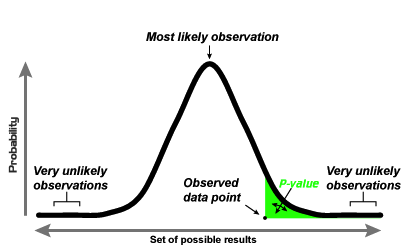
\includegraphics[width=0.4\textwidth]{p_value_one_sided}
  \caption{One sided p-value representation (Author Repapetilto, Wikipedia Foundation Inc)}
  \label{fig:p_value_one_sided}
\end{figure}

Two-sided p-value shows the probability that you get a certain value T that is either larger or smaller than the computed test statistic from the observed data in the distribution that the null-hypothesis defines. This can be seen visually in the Figure ~\ref{fig:p_value_two_sided}.

\begin{figure}[!ht]
  \centering
  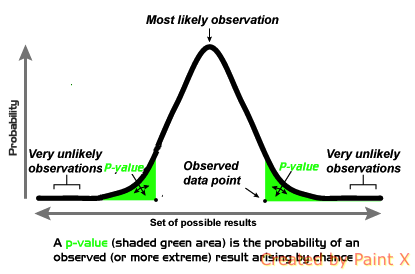
\includegraphics[width=0.4\textwidth]{p_value_two_sided}
  \caption{Two sided p-value representation (Modified by author, source from Wikipedia Foundation inc, Repapetilto)}
  \label{fig:p_value_two_sided}
\end{figure}

\newpage
\subsection{Wilcoxon test}

The Wilcoxon signed-rank test is a statistical hypothesis test that is used when comparing two related samples, matched samples, or repeated measurements on a single sample. This means that with Wilcoxon test you can look at some measurable feature, e.g. blood pressure. If two or more experiments in different conditions have been made on it,e.g. gene experiments and their confirmation results, Wilcoxon test can be used to see if the changes of the measurement levels are relevant. The null hypothesis $H_0$ means that the difference between pairs is zero. The alternative $H_1$ means it is not.

It was popularized by Sidney Siegel in his book "Nonparametric statistics - for the behavioral sciences". Sidney used the symbol $T$, to denote test statistic. Because of this, the test is sometimes referred to as the Wilcoxon T test and the test statistic is reported as a value of $T$.

\newpage

\subsection{Wilcoxon test Assumptions}

\begin{enumerate}
  \item Two measurements can always be compare and thus ordered. For example, measurement is a real value or ordered categorical values
  \item Measurements can be naturally paired into case-control or before-after experiments. For example, measure patients white blood cell levels before and after treatment.
  \item All measurement pairs are independent from other pairs. For example, measurement of one individual does not influence the other. In medicine patients in the study are sampled randomly. There is no evident procedure in selecting patients or no planned action to organize a study so one could get the "desired" result.
\end{enumerate}

\subsection{How to compute}
Let $N$ be the sample size, the number of pairs. Then we can use the following variable to compute the W test. For $i=1,...,N$, let $x_{1, i}$ and $x_{2, i}$ denote the measurements.
Let $W$ be the wilcoxon test statistic.
Let $z-score$ be the wilcoxon test standard score.
Let $N_0$ be the number of pairs from which onward one can approximate the p-value. This value is currently undefined and is the focus of this paper. It will be discussed in the future chapters.

The computation of the statistic W is organised into five steps. The last step diverges into two possible paths and the choice of the path that is chosen depends wether $N  >= N_0$.

\begin{enumerate}
\item
For $i=1, .., N$, calculate $|x_{2,i} - x_{1,i}|$ and $\sign(x_{2,1} - x_{1,i})$, where $\sign(x)$ is the sign function.
\item
Order the $N$ pairs from smallest absolute difference to largest absolute difference, $|x_{2,i} - x_{1,i}|$.
\item
Rank the pairs, starting with the smallest as $1$. Ties receive a rank equal to the average of the ranks they span. Let $R_i$ denote the rank.
\item
Calculate the test statistic $W$, the absolute value of the sum of the signed ranks.
\begin{equation}
  W=|\sum\limits_{i=1}^{N} [\sign(x_{2,i} - x_{1,i})*R_i]|
\end{equation}

\item
As $N$ increases, the sampling distribution of $W$ converges to a gaussian distribution. Where $N_0$ depends on how accurate you want your results to be.
\begin{enumerate}
\item
For $N >= N_0$, a $z-score$ can be calculated as
\begin{equation}
  z=\frac{W-0.5}{\sigma_w},\sigma_w = \sqrt{\frac{N(N + 1)(2N + 1)}{6}}
\end{equation}

If $Z > Zcritical$ then reject $H_0$, where $Z_{critical}$ is calculated with Gaussian distribution.

\item
For $N < N_0$, $W$  is compared to a $p-value$ that can be calculated from enumeration of all possible combinations of $W$ given $N$.

If $W >= P_{critical}$, $N$ then reject $H_0$
\end{enumerate}
\end{enumerate}

\subsection{Example}
Given pairs $(6, 8), ((2, -3), (-3, 3), (1, 3)$.

\begin{enumerate}
\item Calculate absolute values and signs: \\
Absolute values $(2, -5, 6, 2)$ \\
Signs $(1, -1, 1, 1)$
\item Order the pairs. Ties receive therank equal to average of the ranks they span \\
$(2 => 1.5), (5 => 3), (6 => 4), (2 => 1.5)$
\item Calculate the test statistic W \\
$W = 1*1.5+ 1*1.5 + (-1*3) + 1*4 $ = 4.0
\item Since $N_r$ is very small, use a table to look up the $p$ value. The calculation of $p$ table is in a later chapter. \\
$P(5, 4) = 0.3125$ \\
Since $0.3125 > 0.05$, reject $H_1$
\end{enumerate}

The calculations can also be seen on Table ~\ref{table:wilx_example_1} and Table ~\ref{table:wilx_example_2}.

\begin{table}[h!]
  \begin{center}
    \begin{minipage}{.5\linewidth}
      \begin{center}
        \begin{tabular}{ccccc}
          \hline
          i & $x_{2, 1}$ & $x_{1, i}$ & $\sign$ & abs \\
          \hline
          1 & 6 & 8 & 1 & 2 \\
          \hline
          2 & 2 & -3 & -1 & 5 \\
          \hline
          3 & -3 & 3 & 1 & 6 \\
          \hline
          4 & 1 & 3 & 11 & 2 \\
          \hline
        \end{tabular}
        \caption{Initial data}
        \label{table:wilx_example_1}
      \end{center}
    \end{minipage}%
    \begin{minipage}{.5\linewidth}
      \begin{center}
        \begin{tabular}{ccccccc}
          \hline
          i & $x_{2, 1}$ & $x_{1, i}$ & $\sign$ & abs & $R_i$ & $\sign * R_i$ \\
          \hline
          1 & 6 & 8 & 1 & 2 & 1.5 & 1.5\\
          \hline
          4 & 1 & 3 & 11 & 2 & 1.5 & 1.5\\
          \hline
          2 & 2 & -3 & -1 & 5 & 3 & -3 \\
          \hline
          3 & -3 & 3 & 1 & 6 & 4 & 4\\
          \hline
        \end{tabular}
        \caption{After ordering by absolute difference}
        \label{table:wilx_example_2}
      \end{center}
    \end{minipage}%
  \end{center}
\end{table}


\subsection{P-value assignment}
Let us consider Wilcoxon test if we have 6 measurements. Then there are three differences as shown in in Figure ~\ref{fig:patientExample}. As the test considers only the sign and order of the measurements, then only 8 configurations are possible as shown in Figure ~\ref{fig:rankSignsExample} and Table ~\ref{table:adding_w_results}.

The formula to calculate that result was $2^n$. Due to the symmetry of of the possible configurations under the distribution of the null hypothesis, all 8 configurations can be proven equally probable.
\begin{figure}[h!]
  \centering
  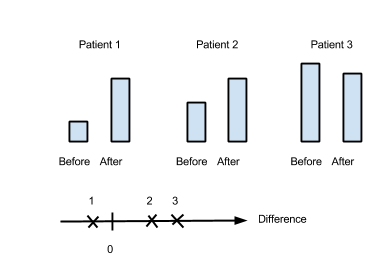
\includegraphics[width=0.8\textwidth]{patientExample}
  \caption{Patient example}
  \label{fig:patientExample}
\end{figure}

\begin{figure}[h!]
  \centering
  
\includegraphics[width=0.8\textwidth]{rankSignsExample}
  \caption{Two sided p-value representation}
  \label{fig:rankSignsExample}
\end{figure}

Now if the W value in our data is +2, then there are 3 configurations that have larger or equal W value. This can be seen from the Table ~\ref{table:adding_w_results}. Then the one-sided p-value is $\frac{3}{8}$. The two-sided p-value is $\frac{3}{4}$. The same procedure is needed to assign p-value.

\begin{table}[!ht]
  \begin{center}
      \begin{tabular}{c}
      \hline
      $W = 1 + 2 + 3 = 6$ \\
      \hline
      $W = -1 + 2 + 3 = 4$\\
      \hline
      $W = -1 - 2 + 3 = 0$\\
      \hline
      $W = 1 - 2 + 3 = 2$\\
      \hline
      \end{tabular}
      \begin{tabular}{c}
      \hline
      $W = -1 - 2 - 3 = -6$\\
      \hline
      $W = 1 - 2 - 3 = -4$\\
      \hline
      $W = 1 + 2 - 3 = 0$\\
      \hline
      $W = -1 + 2 - 3 = -2$\\
      \hline
      \end{tabular}
    \caption{All eight configurations. Values of the test statistic corresponding to the configuration.}
    \label{table:adding_w_results}
  \end{center}
\end{table}

So in the end, since Wilcoxon test neglets the actual value of the tests, then to estimate the p-value, we only need to know the W value and number of tests. No matter the actual value of the test cases, $W$ statistic will always create the same configurations, given a certain $N$.

\subsubsection{V and P example}

Given $N$ is $2$, then ranks are ${0, 1, 2}$, one can combine them into $0 + 1 + 2$ or $0 + 1 - 2$ or $0 - 1 + 2$ or $0 - 1 - 2$. This gives us one way to get $3$, one way to get $1$, one way to get $-1$ and one way to get $-3$

It can now be calculated that the probability that our there is a $0.25\%$ that our value is $3$ or lower and $0.5\%$ that our value is $1$ or lower.

This distribution is the most accurate table you can compare wilcoxon test results on - it shows the exact probability that your tests falls into a certain gaussian distribution range. However, the table is expensive to calculate.

\subsubsection{Exact computation of P-value}
The problem of assigning a $p$-value can be reduced to the following problem. Given a $N$ ranks, we assign + or - sign to each rank randomly. Since the sign distribution is random, then either sign has equal probability to be assigned. For fixed number of ranks $N$, we can consider all $2^n$ possible sign assignements and find out in how many ways we can assign the ranks to get a certain sum $k$. If we do this for every possible $k$, then a $V$-array is formed. It signifies all the possible random signed rank combination sums in an $N$ sized ranked array, where $k$ shows how many times a certain sum was achived. If we calculate $V$-array for every possible number of ranks up to the fixed $N$, then a $V$-table is formed. We can use the $V$-table to look up the how many times a certain sum $k$ was achived, given $N$ ranks. Let $V_{N, k}$ be the number of times a certain sums was achieved.

From this table, the probabaility that $W\geq k$ can be calculated. This value will show that given $N$ ranks with random signs, how probable it is that a sum $k$ is the result. If this process of calculating values is done repeadedly for every possible $N$ and $k$, then a $P$-table forms. The $P$-table shows the probability of every possible sum $k$ appearing given $N$ ranks with random signs. Let $P_{N, k}$ be the function to get the desired $P$ value from that table.

If the $P$-table gets large enough, it will start taking the shape of Guassian distribution. Because of that, given enough ranks, a gaussian distribution can be used to approximate the $P$-table.

\subsubsection{The V and P table formulas}

Given $N$ which shows us the number of ranks starting from $0$ and $k$ which shows us the sum that we are interested in. Recursively apply this algorithm until you reach to the $N = 1$.

\begin{equation}
  V_{N+1, k} = V_{N, k-1} + V_{N, k+N+1}
\end{equation}

There are some additional conditions to the formula:

\begin{equation}
V_{N, k} = 0  \quad\text{if}\quad k < -N  \frac{N+1}{2} \quad\text{or}\quad k > N  \frac{N+1}{2}
\end{equation}

\begin{equation}
V_{N, k} = 1 \quad\text{if}\quad k = -N  \frac{N+1}{2} \quad\text{or}\quad k = N  \frac{N+1}{2}
\end{equation}

With these formulas, the probability that $W$ is a certain value can be calculated.

Given $V$ table, $N$ and $k$, we can calculate the $P$ by

\begin{equation}
P(T) = \frac{1}{2^n} \abs{\sum\limits_{K=T}^{\infty}{W_{N,K}}}
\end{equation}

To get the P table, we go through all $N$ and $K$ values that we are interested in.

\subsubsection{The Gaussian approximation of P table}
As mentioned above, if the number of ranks $N$ gets large enough, then Gaussian distribution can be used. To use that, the cumulative deinsity function $F(x)$ is usually used. A simple Gaussian function function $F(x, 1)$, where $x$ is the statistic $z-value$, eg standard score and $1$ is the sigma, will give approximately the same results as the accurate $P$ table.

\subsubsection{Code sample}
A python code to calculate the V table is as follows:
\begin{verbatim}
def V(n, k, vTable):
    if((n == 1 and (k == 1 or k == -1)) or (n == 0 and k == 0)):
        return 1
    if((k < -(n * (n + 1) / 2)) or (k > (n * (n + 1) / 2))):
        return 0
    n = n - 1

    kIndex =  k + kSize

    leftValue = 0 if kIndex - n - 1 < 0 or \
      kIndex - n - 1 >= len(vTable[n]) else vTable[n][kIndex - n - 1]
    rightValue = 0 if kIndex + n + 1 < 0 or \
      kIndex + n + 1 >= len(vTable[n]) else vTable[n][kIndex + n + 1]

    return leftValue + rightValue

def calculateVValues():
    vTable = []
    for n in range (nSize):
        tableRow = []
        for T0 in range (kSize * 2 + 1):
            tableRow.append(V(n, T0 - kSize, vTable))
        vTable.append(tableRow)
    return vTable

\end{verbatim}

The python code to calculate the P table is as follows:

\begin{verbatim}
def calculatePValues(vTable):
    pTable = []
    for n in range(nSize):
        tableRow = []
        sumValue = 0
        powerValue = 2**n
        for T0 in range (kSize * 2, kSize-1, -1):
            sumValue += vTable[n][T0]
            p = sumValue / powerValue
            tableRow.insert(0, p)
        pTable.append(tableRow)
    return pTable

\end{verbatim}

You can find a python implementation of a code sample in
\url{https://github.com/stenver/wilcoxon-test/blob/master/WilcoxonVTable/pAccurateTable.py}

\subsubsection{Bonferroni correction}

If you make multiple hypothesis on a test, then you increase the risk in which you reject null hypotheses when its actually true. The Bonferroni test helps to counteract this in a simple and naive way. For each hypothesis you make on a test, you should use a significance level $M$ times lower than before. This ensures that the the increased risk in which we can reject null hypothesis will not raise, no matter the number of hypothesis on a test. So for example, if you make $M$ hypothesis and want want a significance level $\alpha$,  then you should run each test at a significance level of $\frac{\alpha}{M}$.

If you want to use Bonferron correction with Wilcoxon signed-rank test, then you need to keep in mind that the approximated $P$ value significance level needs to be much more accurate, since the bonferron test divides it by the amount of features tested. This means higher the $N_0$ value, the more features you add in the test.

\newpage

\section{Approximating the p-value}

\subsection{Motivation}
The current implementations of Wilcoxon signed-rank test usually assume that $p$-value distribution is sufficiently close to Gaussian distribution, so that we can use $Z$ to calculate the $P$ value. They draw this conclusion from the assumption that $N$ is sufficiently large to use $Z$. This allows them to use Gaussian Distributions to approximate the $P$ value and the accurate $P$ table calculation is often left unoptimized. In this work we studied the question whether this assumption is justified in detail.

In the BIIT research group, however, the $N$ is usually not sufficiently large. This means that Gaussian distribution cannot be used. Furthermore, it is not known where exactly the $N$ limit is, so an arbitrary number is used for that purpose. The textbooks~\cite{lowry_concepts} currently suggest a sufficient $N$ is 10.

Also, since BIIT uses multiple hypothesis testing, the approximation must be good even for small P-values. As mentioned above, the Bonferroni correction will lower the $P$ significantly.

Because of this, one focus of the paper is finding out how good the approximation of Gaussian Distribution is. The reason to find it out is, as mention, because approximation is computationally cheap and the preffered method to be used over accurate $P$ table, which is computationally expensive.

\subsection{Approximation traits}
When $N = 1$, then approximation is quite unaccurate. As $N$ increases, then the approximation becomes more and more accurate.

When the $N->\infty$, then the approximate region will almost equal the accurate $P$ region. This means that when $N->\infty$, then there is no reason not to use Gaussian Distribution, as it will be completely accurate.

\subsection{Optimizing}

The bottleneck of the other implementations of the Wilcoxon test, when $N$ is low, is that they calculate the $P$ and $V$ tables every time the test is run, thus if you run thousands of tests in a row, a lot of complex recomputation is done. This eventually becomes a performance issue.

To speed this up - this project will calculate the entire $P_{N, k}$ for every value that is possible where $N < N_0$. Then the $P_{N, k}$ will be hardcoded inside the program for quick lookup of the value.

One of the focuses of this paper is finding the $N_0$ value

\newpage

\section{Finding the $N_0$ value}
\subsection{Proving that $P$ and $P_{approx}$ get more similar as $N$ increases}
First we wanted to confirm that as $N$ grows, $P$ and $P_{approx}$ value will get more and more similar. To do this, we took $P_{N, k}$ value for each $N$ where
$N < 50$ and $P_{N, k}  = 0$ and $P_{N, k - 1} != 0$.
We then compared the $P_{N, k}$ and $P_{approx} (N, k)$ for each $N$ where:
The results are on Figure ~\ref{fig:T0vsN}.


\begin{figure}[!ht]
	\centering
  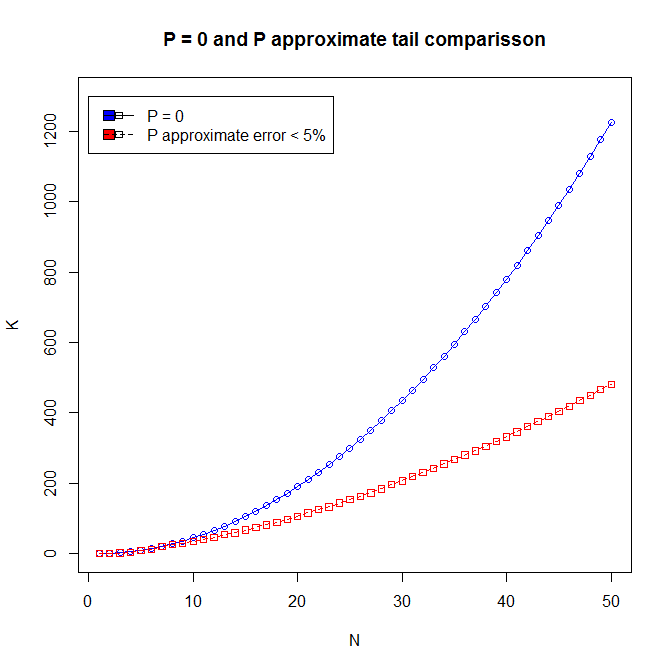
\includegraphics[width=0.8\textwidth]{T0vsN}
	\caption{Approximate and accurate comparisson}
	\label{fig:T0vsN}
\end{figure}

\begin{figure}[!ht]
	\centering
  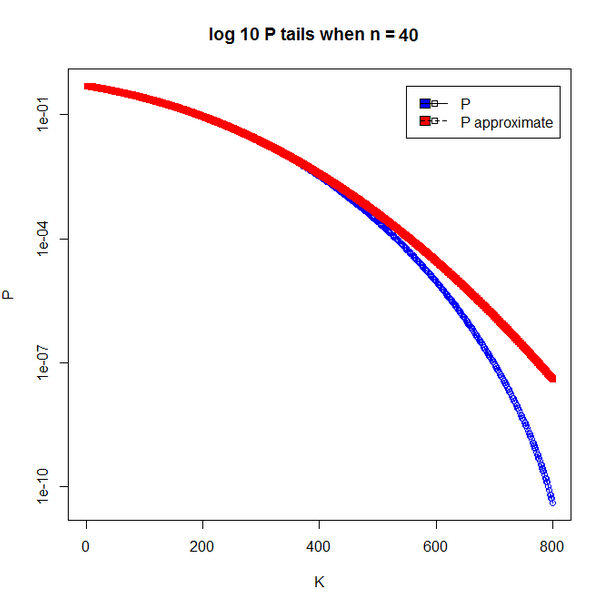
\includegraphics[width=0.8\textwidth]{log10PtailsN40}
	\caption{Relative error increasing toward edge of tail}
	\label{fig:log10PtailsN40}
\end{figure}

Much to our surprise, as $N$ grew, the gap between approximate and accurate $P$ values grew bigger. This meant that as $N$ grows, the Gaussian distribution will get more inaccurate toward the tails of the distribution. Previously we thought that with the growth of $N$, Gaussian would surely get more and more accurate.
From Figure ~\ref{fig:log10PtailsN40} we can see that Gaussian distribution is a little bit bigger and gets bigger as $K$ grows. Figure 2 illustrates the difference in position of between last accurate $P_{appox}$ and $P = 0$. Accurate means that the relvative error is under $5\%$

To further investigate this finding, we decided to find out the minimum $P$ value that you can get for each $N$ while maintaining a certain error threshold. The thresholds chosen were $5\%, 10\%, 20\%, 50\%$. The formula used was the same as before, except the thresholds were replaced as needed.

\begin{figure}[!ht]
	\centering
  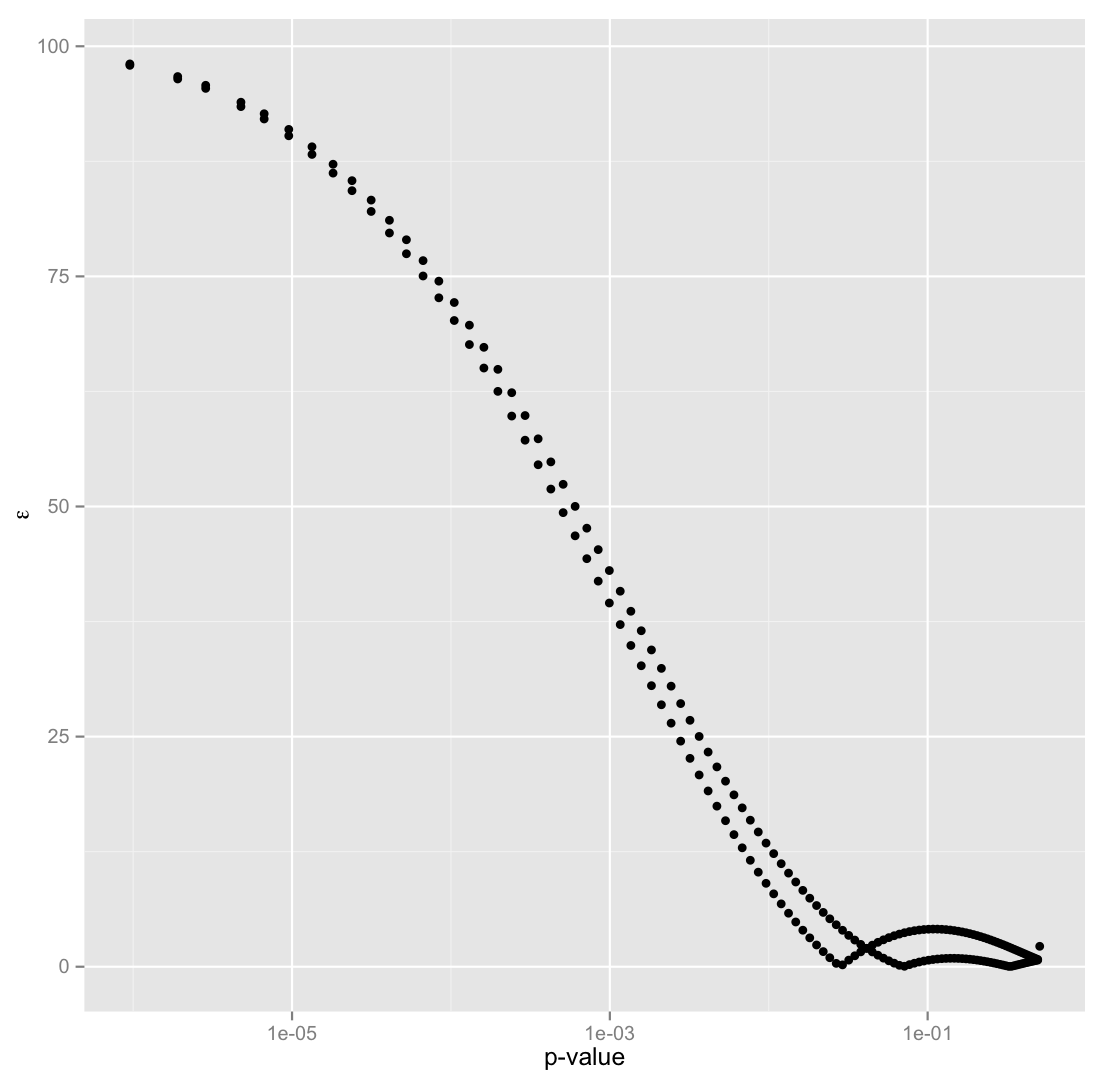
\includegraphics[width=0.8\textwidth]{RelativeErrorDecreasingPgrowsN20}
	\caption{Comparing approximate probability relative error as sample size increses}
	\label{fig:PvsN}
\end{figure}

\begin{figure}[!ht]
	\centering
  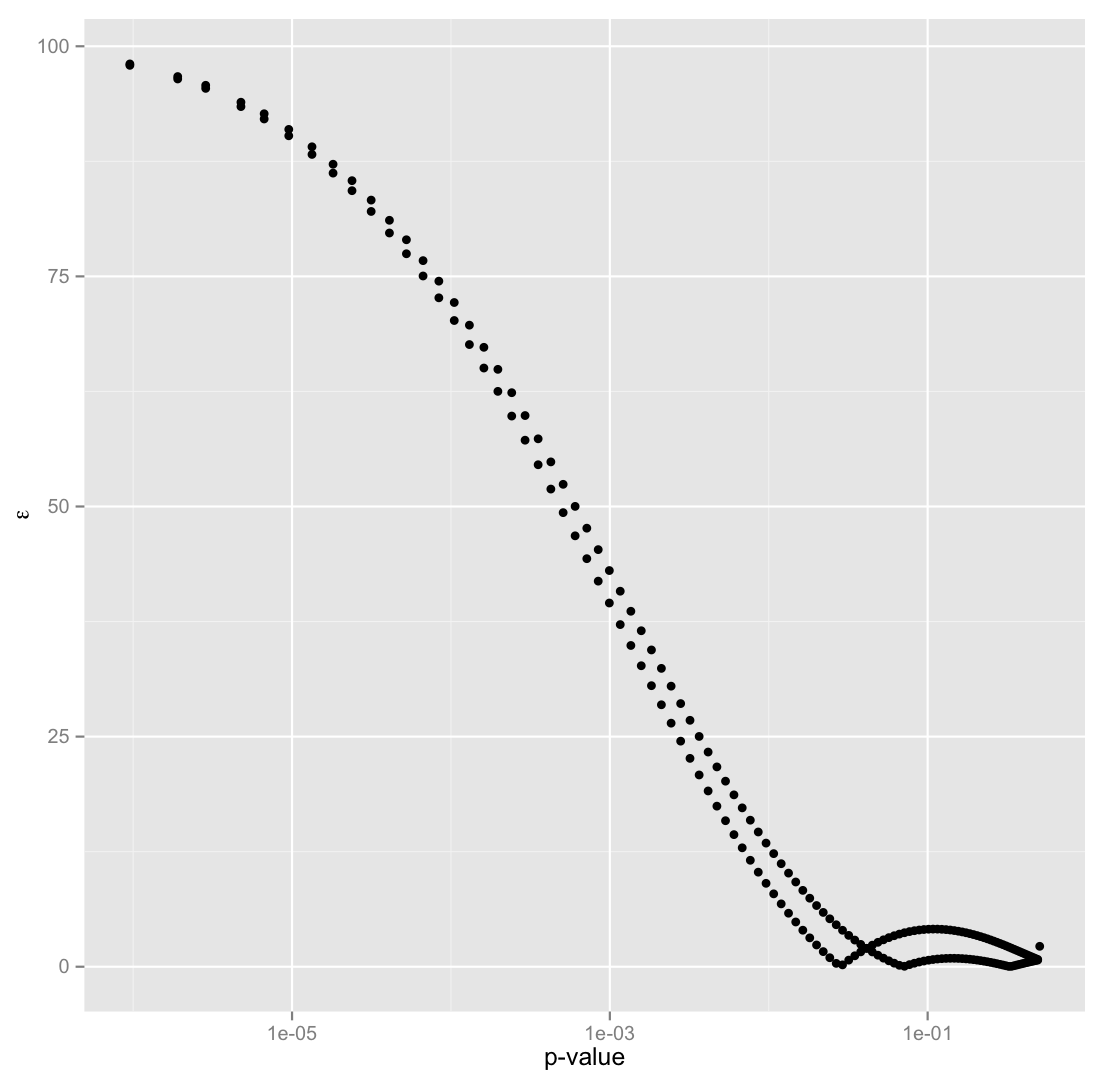
\includegraphics[width=0.8\textwidth]{RelativeErrorDecreasingPgrowsN20}
	\caption{Showing the relative error as probabilty increases when sample size is 20}
	\label{fig:RelativeErrorDecresingPgrows}
\end{figure}

From Figure ~\ref{fig:PvsN} we can see that as the $N$ grows, the graph becomes stable, meaning that the distribution becomes a Gaussian distribution at around $N > 10$ and $N < 25$. We can see that the minimum $P$ value under error threshold does get smaller, as $N$ increases, so this further proves that Gaussian distribution does get more accurate as $N$ grows. This is because as $N$ increases, you can take a $P$ value closer to the tail of the distribution and still get an accurate value.

The Figure ~\ref{fig:RelativeErrorDecresingPgrows} shows us the relative error as $P$ grows when $N = 20$. The $P$ values are logged on this graph. There are two noteworthy things here, however. First, around $P = 0.05$, the relative error actually get a little small tip toward accuracy. Second, it can be seen that there are two accuracy paths that the error takes, depending on weather in $P_{approx N, K}$  the $K$ is even or odd number. This is a computational artefact caused by the recurrence of the $V_{N, K}$ values and we will not make any conclusions of that.

\subsection{Investigating the $P_{N, k}$ and $P_{approx N, K}$ similarities}
To further prove that we can start using Gaussian Distribution at a certain $N$, we needed to prove that Papprox will get more accurate as the N increases toward the tail of the distribution aswell.

To achive this, we found out the largest relative error between $P$ and $P_{approx}$ for each $N$ and for each $P$ where $P = (0.5:0.1), P = (0.1, 0.01), P = (0.001, 0.0001), ... , P = (10-14 , 10-15)$

\begin{figure*}
	\centering
  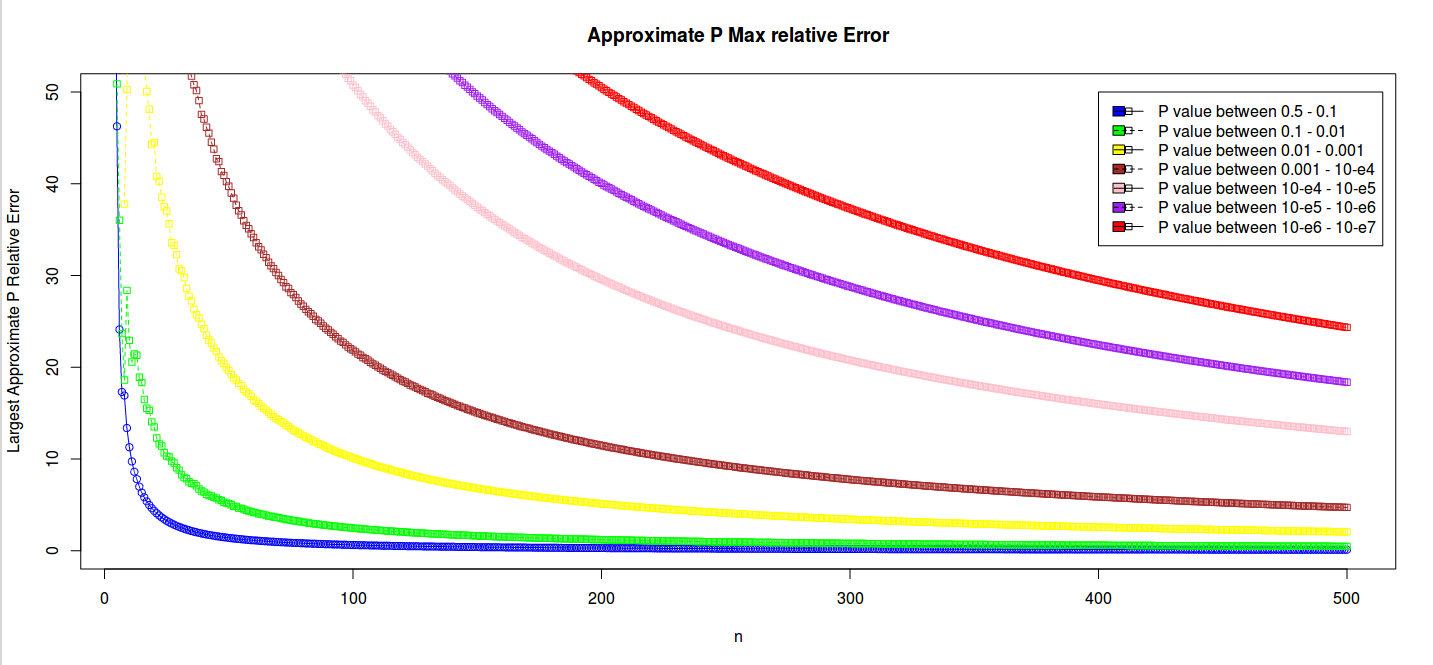
\includegraphics[width=0.8\textwidth]{LargestApproxPRelativeError3}
	\caption{Showing the maximum approximate relative error in probability ranges, as sample size increases}
	\label{fig:LargestApproxPRelativeError}
\end{figure*}

As can be seen from Figure ~\ref{fig:LargestApproxPRelativeError}, the relative error increases exponentially. When $P = (10-5 , 10-6)$ the relative error is massive. When $N=200$, then the error is still around $40\%$. The bigger the $N$ gets, the bigger the error at the tail. However, it can also be seen that the error decreases steadily as $N$ grows for each of the $P$ range chosen.

This means that even though the error of the distribution tail edge does increase as N grows, overall, both distributions get more and more similar to the Gaussian distribution

To further investigate the relation between $P_{N, k}$ and $P_{approx N, K}$, we wanted to see the difference between all $P$ values when $P = 50$ and when $P = 25$

\begin{figure}
	\centering
  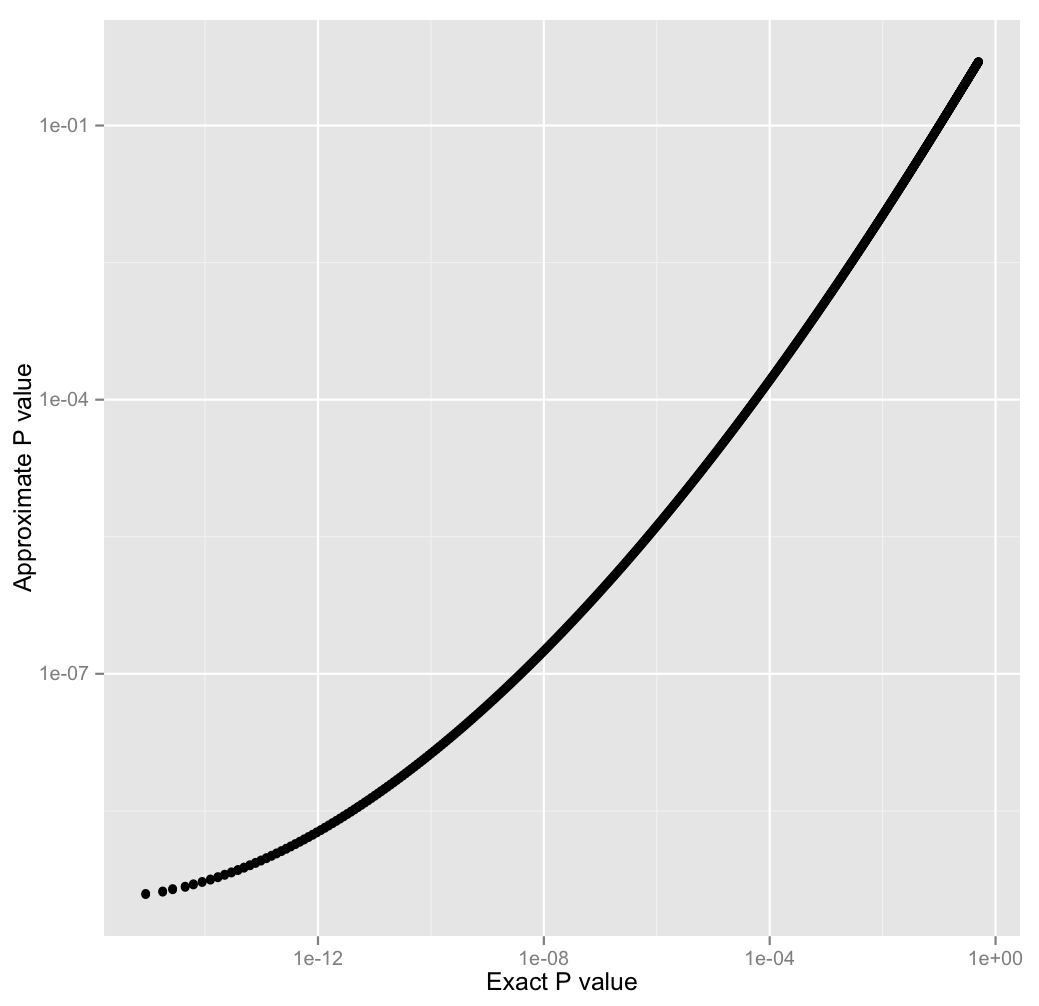
\includegraphics[width=0.8\textwidth]{PvsP50}
	\caption{Relative value of all actual probabilities and approximated probabilities when sample size is 50}
	\label{fig:PvsP50}
\end{figure}

\begin{figure}
	\centering
  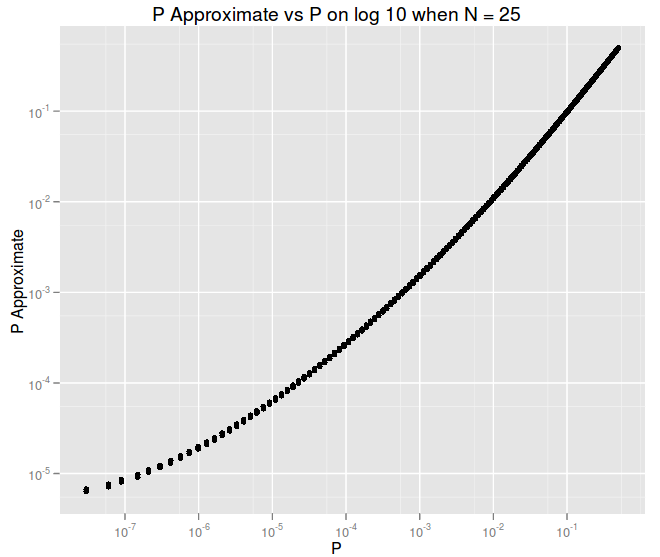
\includegraphics[width=0.8\textwidth]{PvsP25}
	\caption{Relative value of all actual probabilities and approximated probabilities when sample size is 25}
	\label{fig:PvsP25}
\end{figure}

As can be seen from Figure ~\ref{fig:PvsP50} or Figure ~\ref{fig:PvsP25}, when the $N = 50$ or $N = 25$, then the $P_{N, k}$ and $P_{approx N, K}$ values are almost the same with slight differences - the $P_{approximate}$ is a little bit larger. When $N = 25$, the graph is a little less smooth, which tells us that the differences are not as similar as they are when $N = 50$.

\subsection{Determining the $N_0$ value}
Judging by all the data that has been gathered, it be can clearly see that as $N$ grows, $P_{N, k}$ and $P_{approx N, K}$ tail edges grow apart but overall the distribution gets more and more similar. Determining the $N_0$ value depends on the amount of data we have and the accuracy of the result we want. The most helpful graphs to help us determine the necessary $N_0$ value is Figure ~\ref{fig:LargestApproxPRelativeError}. Table ~\ref{table:requiredN} illustrates the number of samples($N$) needed for a certain relative accuaracy. So the $N_0$ value depends on the number of measurements and the required accuracy where $N_0 = N$:

\begin{table}[!ht]
	\begin{center}
		\caption{Showing the minimal required sample size for a certain relative error and number of measurements}
	    \begin{tabular}{| l | l | l |}
	    \hline
		Measurements & Error & Required N \\
		\hline
		10 & 5\% & 25 \\
		100 & & 250 \\
		1000 & & 500 \\
		10000 & & $>500$ \\
		100000 & & $> 500$ \\
		\hline
		10  & 10\% & 80 \\
		100 & & 200 \\
		1000 & & $>500$ \\
		10000 & & $>500$ \\
		100000  & & $>500$ \\
		\hline
		10  & 20\% & 50 \\
		100 & & 100 \\
		1000  & & 280 \\
		10000  & & 500 \\
		100000  & & $>500$ \\
		\hline
		10  & 50\% &  25 \\
		100 & & 50 \\
		1000 & & 100 \\
		10000 & & 150 \\
		100000 & & 200 \\
		\hline
		\end{tabular}
		\label{table:requiredN}
	\end{center}
\end{table}

As pointed out in the beginning, when the $N$ grows, the $P_{N, k}$ table size grows exponentially.

Since even when $N = 80$, the plain text file was already 2.5mb, the need to optimize further arised.

\section{Further optimizations}

To further optimize the library, it was needed to approximate the accurate $P$ table. Two algorithms were chosen for that matter dose-response curve and linear approximation.

\subsubsection{dose-response curve}
When using the dose-reponse curve algorithm, the data range as shown in Figure~\ref{fig:PdivPapproxDrcWhenN500} changes sharply toward the edge of the range. Further tests also showed that the algorithm was completly inaccurate at the end of the far edge, so unfortunately this algorithm could not be used.

\begin{figure}
  \centering
  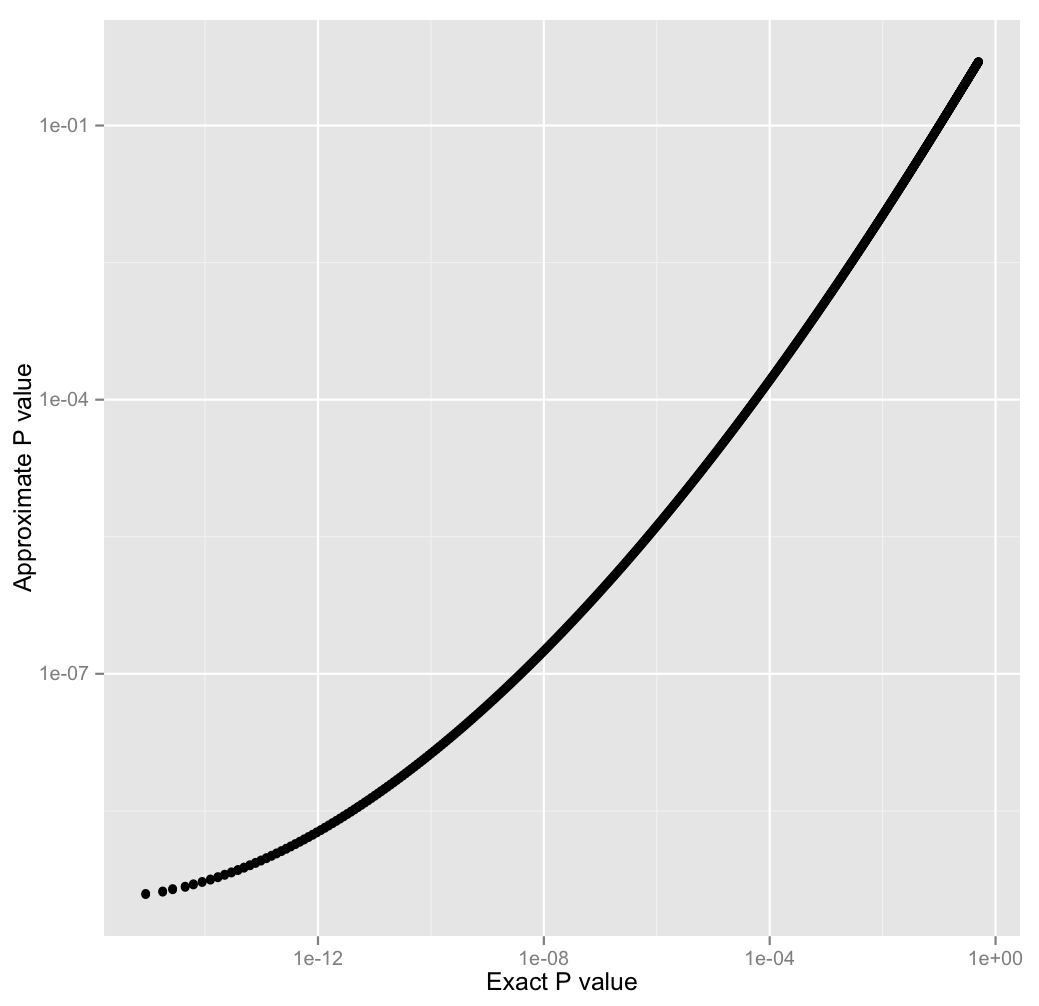
\includegraphics[width=0.8\textwidth]{PvsP50}
  \caption{P range with DRC algorithm when N=500}
  \label{fig:PdivPapproxDrcWhenN500}
\end{figure}

\subsection{Linear approximation}

A more straight forward algorithm to use was linear approximation. The tests showed that using relative $P$ values between the $P$ tables gave less approximated data points, then using straight forward accurate $P$ table.

\subsubsection{Relative values between P tables}

The algorithm to get a relative value for every position between the P tables was pretty straight forward. In Python it looked like this:

\begin{verbatim}
def getRelativeValuesInRow(n, pTable, gaussianPTable):
    pRelativeValues = []
    for j in range(len(pTable[n])):
      relativeValue = pTable[n][j] / gaussianPTable[n][j]
      pRelativeValues.append(relativeValue)
      if(pTable[n][j] == 0):
          break
    return pRelativeValues

def calculateRelativeTable(pTable, gaussianPTable):
  relativeTable = []
  for n in range(len(pTable)):
    relativeTable = getRelativeValuesInRow(n, pTable, gaussianPTable)
  return relativeTable

\end{verbatim}

This returned a new table which had the same number of elements as the accurate P table or Guassian P rable, but for every position there was a relative p-value.

\subsubsection{Linear approximation algorithm}

The linear approximation algorithm works by starting from data point in the data range and then one by one moving to the next data point, until the points between them cannot be approximated with enough accuracy. Then the last accurate point is saved, picked as the next starting point and the process is repeated until end of range has been reached. This guarantees approximated data range within error margin.

The to approximate the data points in python look like this
\newpage
\begin{verbatim}
def linearInterpolate(approximatePoint,
                      endPoint,
                      startPoint,
                      endValue,
                      startValue):
  return startValue +
          ((endValue - startValue) * (approximatePoint - startPoint) /
          (endPoint - startPoint))

def canApproximate(actualPoints, currentPoint, nextPoint):
  startValue = actualPoints[currentPoint]
  endValue = actualPoints[nextPoint]

  for i in range(1, nextPoint - currentPoint):
    approximatePoint = currentPoint + i
    trueValue = actualPoints[approximatePoint]
    approximateValue = linearInterpolate(approximatePoint,
                                          currentPoint,
                                          nextPoint,
                                          startValue,
                                          endValue)
    if approximateValue == 0:
      return True

    relativeAccuaracy = trueValue / approximateValue

    if relativeAccuaracy < 0.9 or relativeAccuaracy > 1.1:
      return False
  return True

def getNextApproximatedPoint(actualPoints, currentPoint):
  nextPoint = currentPoint + 1

  while(canApproximate(actualPoints, currentPoint, nextPoint)):
    if(nextPoint == len(actualPoints) - 1):
      break
    nextPoint += 1
  return nextPoint

def calculateApproximateRow(actualPoints):
  approximatedPoints = []
  currentPoint = 0
  approximatedPoints.append([currentPoint, actualPoints[currentPoint]])

  while(currentPoint != len(actualPoints) - 1):
    nextPoint = getNextApproximatedPoint(actualPoints, currentPoint)
    approximatedPoints.append([nextPoint, actualPoints[nextPoint]])
    currentPoint = nextPoint
  return approximatedPoints

\end{verbatim}

\subsubsection{Linear interpolation}
To reverse the algorithm, a very simple formula - linear interpolation is used. Given the approximate $x$, start point $x_1$, end point $x_2$, start point $y_1$, end point $y_2$, you can easily approximate the $y$ of that point.

$y = y_1 + \frac{(y_2 - y_1) * (x - x_1)}{(x_2 - x_1)}$

In python the code looks like this:

\begin{verbatim}
def linearInterpolate(approximatePoint,
                      endPoint,
                      startPoint,
                      endValue,
                      startValue):
  return startValue +
          ((endValue - startValue) * (approximatePoint - startPoint) /
          (endPoint - startPoint))
\end{verbatim}

\subsection{Optimization summary}
In the end, thanks to linear approximation, the approximated table, when $N=500$ could be created. The error margin for the chosen approximated table was chosen to be $20\%$, since that was deemed as accurate enough. Its still a lot more accurate then Gaussian P table at the edges of the table.

The approximated table is only 1.6mb large. Smaller then when $N=80$ the accurate P table was.

As for the library itself - it could run over 20000 wilcoxon tests with 120 samples in under 0.7 seconds. Compared to the vanilla R implementation which took many seconds to run 20 tests, this is a significant improvement.

\subsection{Further optimizations}
A lot of further optimizations could be done on this subject, for example

\begin{enumerate}
\item The algorithm to approximate accurate P table could be improved.
\item The plain text file could be compressed.
\item The shared library algorithm implementations could be improved and expanded.
\end{enumerate}

\newpage

\section{The implementaion}
Repository that contains everything about our findings can be found in

\url{https://bitbucket.org/stenver/wilxoni-astaku-test/src/870cc6112d0d?at=default} repository

The repository contains a number of folders.

\subsection{RcppWilcoxonTest}
 An interface that connects our implementation of the optimized Wilcoxon algorithm to the R. Note that you must have installed our implementation to use it. The interface must be compiled with separate R commands from the command line. You need Rcpp packages for R to use it. It can be installed in R console by running:

\begin{lstlisting}
$install.packages("Rcpp")
\end{lstlisting}

After that, the package can be installed to R by running the command in the command line in the folder:

\begin{lstlisting}
$R CMD INSTALL .
\end{lstlisting}

You can now load our library in R by calling the

\begin{lstlisting}
>library('RcppWilcoxonTest')
\end{lstlisting}

and you invoke the function by calling

\begin{lstlisting}
>RcppWilcoxonTest::WilxTest(dataMatrix, testIndexes, controlIndexes)
\end{lstlisting}

\subsection{TerminalWilcoxonTest}

An interface that connects our implementation of the optimized Wilcoxon algorithm to the R. Note that you must have installed our implementation to use it. The interface can be compiled by going to the folder, compiling and running help for further help.

\begin{lstlisting}
$make
WilcoxonTest --help
\end{lstlisting}

Currently only supports NetCDF file as input data.

\subsection{WilcoxonTestLibrary}
Implementation for the optimized wilcoxon test. The library can be installed by going to the folder and running

\begin{lstlisting}
make install
\end{lstlisting}

\subsection{WilcoxonVTable}
Python program that can calculate $V$, $P$ and approximated $P$ tables, print them, create files of the tables and create a number of graphs on the tables.

\subsection{Seminar\_paper}
The folder that contains this paper and all images attached to it. It also contains R programs to create those images.

\newpage

\section{Conclusion}
It was found out that Gaussian distribution tail edge grows larger apart from the $P_{N, k}$ as $N$ increases while the overall distribution grows more similar. In addition, it was confirmed that if thousands of parallel tests are ran, then using approximation is not reliable and instead an accurate table of p-values must be used. Calculating that table is very expensive and thus it is advised to precalculate the table for the program. However, the research shows that if 10 000 measurements are run under 5\% relative error, then the hardcoded $N$ should be over 1000. Table of that size would take many gigabytes of space and is impractical to use.

To get around that, approximation of the accurate $P$ table was used. This allowed to significantly reduce the size of the file and thus increase the hardcoded $N$ that was implemented inside the library.

For the time being, the chosen $N$ was 500, with $20\%$ error margin on the approximation. This is still significantly more accurate then Gaussian approximated table at the edges of the distribution. It will allow to make 1000 parallel measurement with 5\% error margin.

The library itself could run over 20000 parallel tests with 100 samples in under a second. It is a shared C++ library with currently implemented interfaces in Cron R and Terminal.

Overall the research included some surprising results and can be considered a success.

\newpage

\selectlanguage{estonian}

\section{Eestikeelne pealkiri}
Bakalaureusetöö(6 EAP) \\
Eesnimi Perekonnanimi \\
Resümee \\


\selectlanguage{english}

\newpage

\bibliographystyle{alpha}
\bibliography{bachelor-thesis}

\appendix
\pagebreak

\section*{\small Non-exclusive licence to reproduce thesis and make thesis public}

I, Stenver Jerkku (date of birth: 10th of October 1990),

\begin{tabbing}
\= Xiii\=\kill
\>1. \> herewith grant the University of Tartu a free permit (non-exclusive licence) to:\\\\

\>1.1\>
\begin{minipage}[t]{14.2cm}
reproduce, for the purpose of preservation and making available to the public, including for addition to the DSpace digital archives until expiry of the term of validity of the copyright, and
\end{minipage}
\\\\
\>1.2
\begin{minipage}[t]{14.2cm}
make available to the public via the web environment of the University of Tartu, including via the DSpace digital archives until expiry of the term of validity of the copyright,\\

Paralell Wilcoxon Signed-rank tests\\

supervised by Sven Laur

\end{minipage}\\\\
\>2. \>I am aware of the fact that the author retains these rights.\\\\
\>3. \>
\begin{minipage}[t]{14.2cm}
I certify that granting the non-exclusive licence does not infringe the intellectual property rights or rights arising from the Personal Data Protection Act.
\end{minipage}\\
\end{tabbing}

\noindent
Tartu, 14.05.2014

\end{document}
